\chapter{System Functionality}

\section{Introduction}
This chapter describes the core aspects of the system's functionality, covering its architecture, primary functions, planning, and testing results that define the application’s capabilities. The first part explains the system’s architecture, and the second part details the main functionalities.

\section{System Architecture}
\begin{figure}[!h]
    \centering
    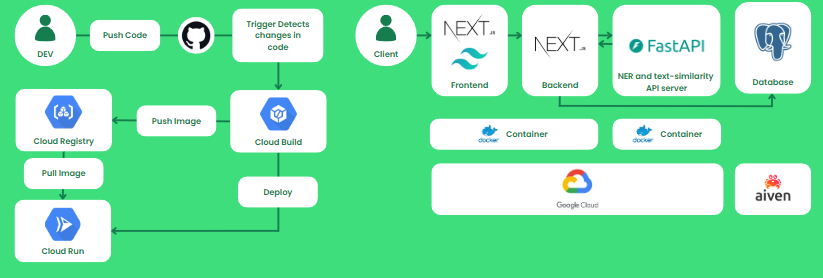
\includegraphics[width=1\linewidth]{chapter4/sysarch.png}
    \caption{System Architecture}
    \label{fig:System Architecture}
\end{figure}
The system architecture consists of two main components designed to deliver an efficient lost-and-found platform. The front end, developed using Next.js, serves as the user interface for tasks like reporting lost items and browsing found items. It communicates with the backend via REST APIs and is containerized using Docker, deployed on Google Cloud Run for scalability. The backend, also built with Next.js and integrated with FastAPI, handles advanced functionalities like Natural Entity Recognition (NER) and text similarity algorithms to automate item matching. Data is managed using a PostgreSQL database hosted on Aiven, ensuring reliable and secure storage. The deployment process is streamlined with a CI/CD pipeline using Google Cloud Build, which automatically builds and deploys container images to Cloud Run, enabling an agile and scalable system.

\needspace{10\baselineskip}
\section{Test Plan and Results}
\begin{table}[h!]
\centering
\begin{tabular}{|l|p{4cm}|p{4cm}|l|}
\hline
\textbf{Module} & \textbf{Test Description} & \textbf{Expectation} & \textbf{Result} \\
\hline
Authentication & Login with Microsoft Azure & Can log in with the KMUTT account & Success \\
\hline
Home Page & Navigate to Lost Report and Found Report forms & Can navigate to both forms & Success \\
\hline
Home Page & Navigate to the user profile page & Correct navigation to profile page & Success \\
\hline
Home Page & Log out from the profile & User logged out successfully & Success \\
\hline
Create Report Form & Fill in the form & Form is successfully filled and submitted & Success \\
\hline
Create Report Form & Validate required fields & Shows error for missing mandatory fields & Success \\
\hline
Create Report Form & Submit the report form & Report saved and reflected in the database & Success \\
\hline
Matching Process & Match lost items to found items & Matches displayed correctly with similarity score & Success \\
\hline
Matching Process & Display contact information of matched user & Contact information displayed correctly & Success \\
\hline
History Log & View previous reports filed by the user & Complete list of past reports displayed & Success \\
\hline
User Profile & Update user information (e.g., phone number) & User information updated successfully & Success \\
\hline
\end{tabular}
\caption{Test Plan and Results}
\end{table}

% \section{System Functions}
% The system supports the following core functionalities:
% \begin{enumerate}
%     \item \textbf{Authentication:} Users log in using their KMUTT email accounts via Microsoft Azure authentication.
%     \item \textbf{Lost \& Found Reporting:} Users can report lost or found items, specifying descriptions, locations, and timestamps.
%     \item \textbf{Item Matching:} Advanced algorithms like NLP and text similarity are used to compare descriptions of lost and found items.
%     \item \textbf{Notification System:} Users receive timely alerts about potential matches or reminders to retrieve items.
%     \item \textbf{History Log:} A record of past reports and claims is maintained for user reference.
%     \item \textbf{Profile Management:} Users can update personal information, such as contact details, through the platform.
% \end{enumerate}
